\documentclass[11pt,a4paper]{report}
\usepackage[textwidth=37em,vmargin=30mm]{geometry}
\usepackage{calc,xunicode,amsmath,amssymb,paralist,enumitem,tabu,booktabs,datetime2,xeCJK,xeCJKfntef,listings}
\usepackage{tocloft,fancyhdr,tcolorbox,xcolor,graphicx,eso-pic,xltxtra,xelatexemoji}

\newcommand{\envyear}[0]{2025}
\newcommand{\envdatestr}[0]{2025-05-07}
\newcommand{\envfinaldir}[0]{webdb/2025/20250507/final}

\usepackage[hidelinks]{hyperref}
\hypersetup{
    colorlinks=false,
    pdfpagemode=FullScreen,
    pdftitle={Web Digest - \envdatestr}
}

\setlength{\cftbeforechapskip}{10pt}
\renewcommand{\cftchapfont}{\rmfamily\bfseries\large\raggedright}
\setlength{\cftbeforesecskip}{2pt}
\renewcommand{\cftsecfont}{\sffamily\small\raggedright}

\setdefaultleftmargin{2em}{2em}{1em}{1em}{1em}{1em}

\usepackage{xeCJK,xeCJKfntef}
\xeCJKsetup{PunctStyle=plain,RubberPunctSkip=false,CJKglue=\strut\hskip 0pt plus 0.1em minus 0.05em,CJKecglue=\strut\hskip 0.22em plus 0.2em}
\XeTeXlinebreaklocale "zh"
\XeTeXlinebreakskip = 0pt


\setmainfont{Brygada 1918}
\setromanfont{Brygada 1918}
\setsansfont{IBM Plex Sans}
\setmonofont{JetBrains Mono NL}
\setCJKmainfont{Noto Serif CJK SC}
\setCJKromanfont{Noto Serif CJK SC}
\setCJKsansfont{Noto Sans CJK SC}
\setCJKmonofont{Noto Sans CJK SC}

\setlength{\parindent}{0pt}
\setlength{\parskip}{8pt}
\linespread{1.15}

\lstset{
	basicstyle=\ttfamily\footnotesize,
	numbersep=5pt,
	backgroundcolor=\color{black!5},
	showspaces=false,
	showstringspaces=false,
	showtabs=false,
	tabsize=2,
	captionpos=b,
	breaklines=true,
	breakatwhitespace=true,
	breakautoindent=true,
	linewidth=\textwidth
}






\newcommand{\coverpic}[2]{
    % argv: itemurl, authorname
    Cover photo by #2~~(\href{#1}{#1})
}
\newcommand{\makeheader}[0]{
    \begin{titlepage}
        % \newgeometry{hmargin=15mm,tmargin=21mm,bmargin=12mm}
        \begin{center}
            
            \rmfamily\scshape
            \fontspec{BaskervilleF}
            \fontspec{Old Standard}
            \fontsize{59pt}{70pt}\selectfont
            WEB\hfill DIGEST
            
            \vfill
            % \vskip 30pt
            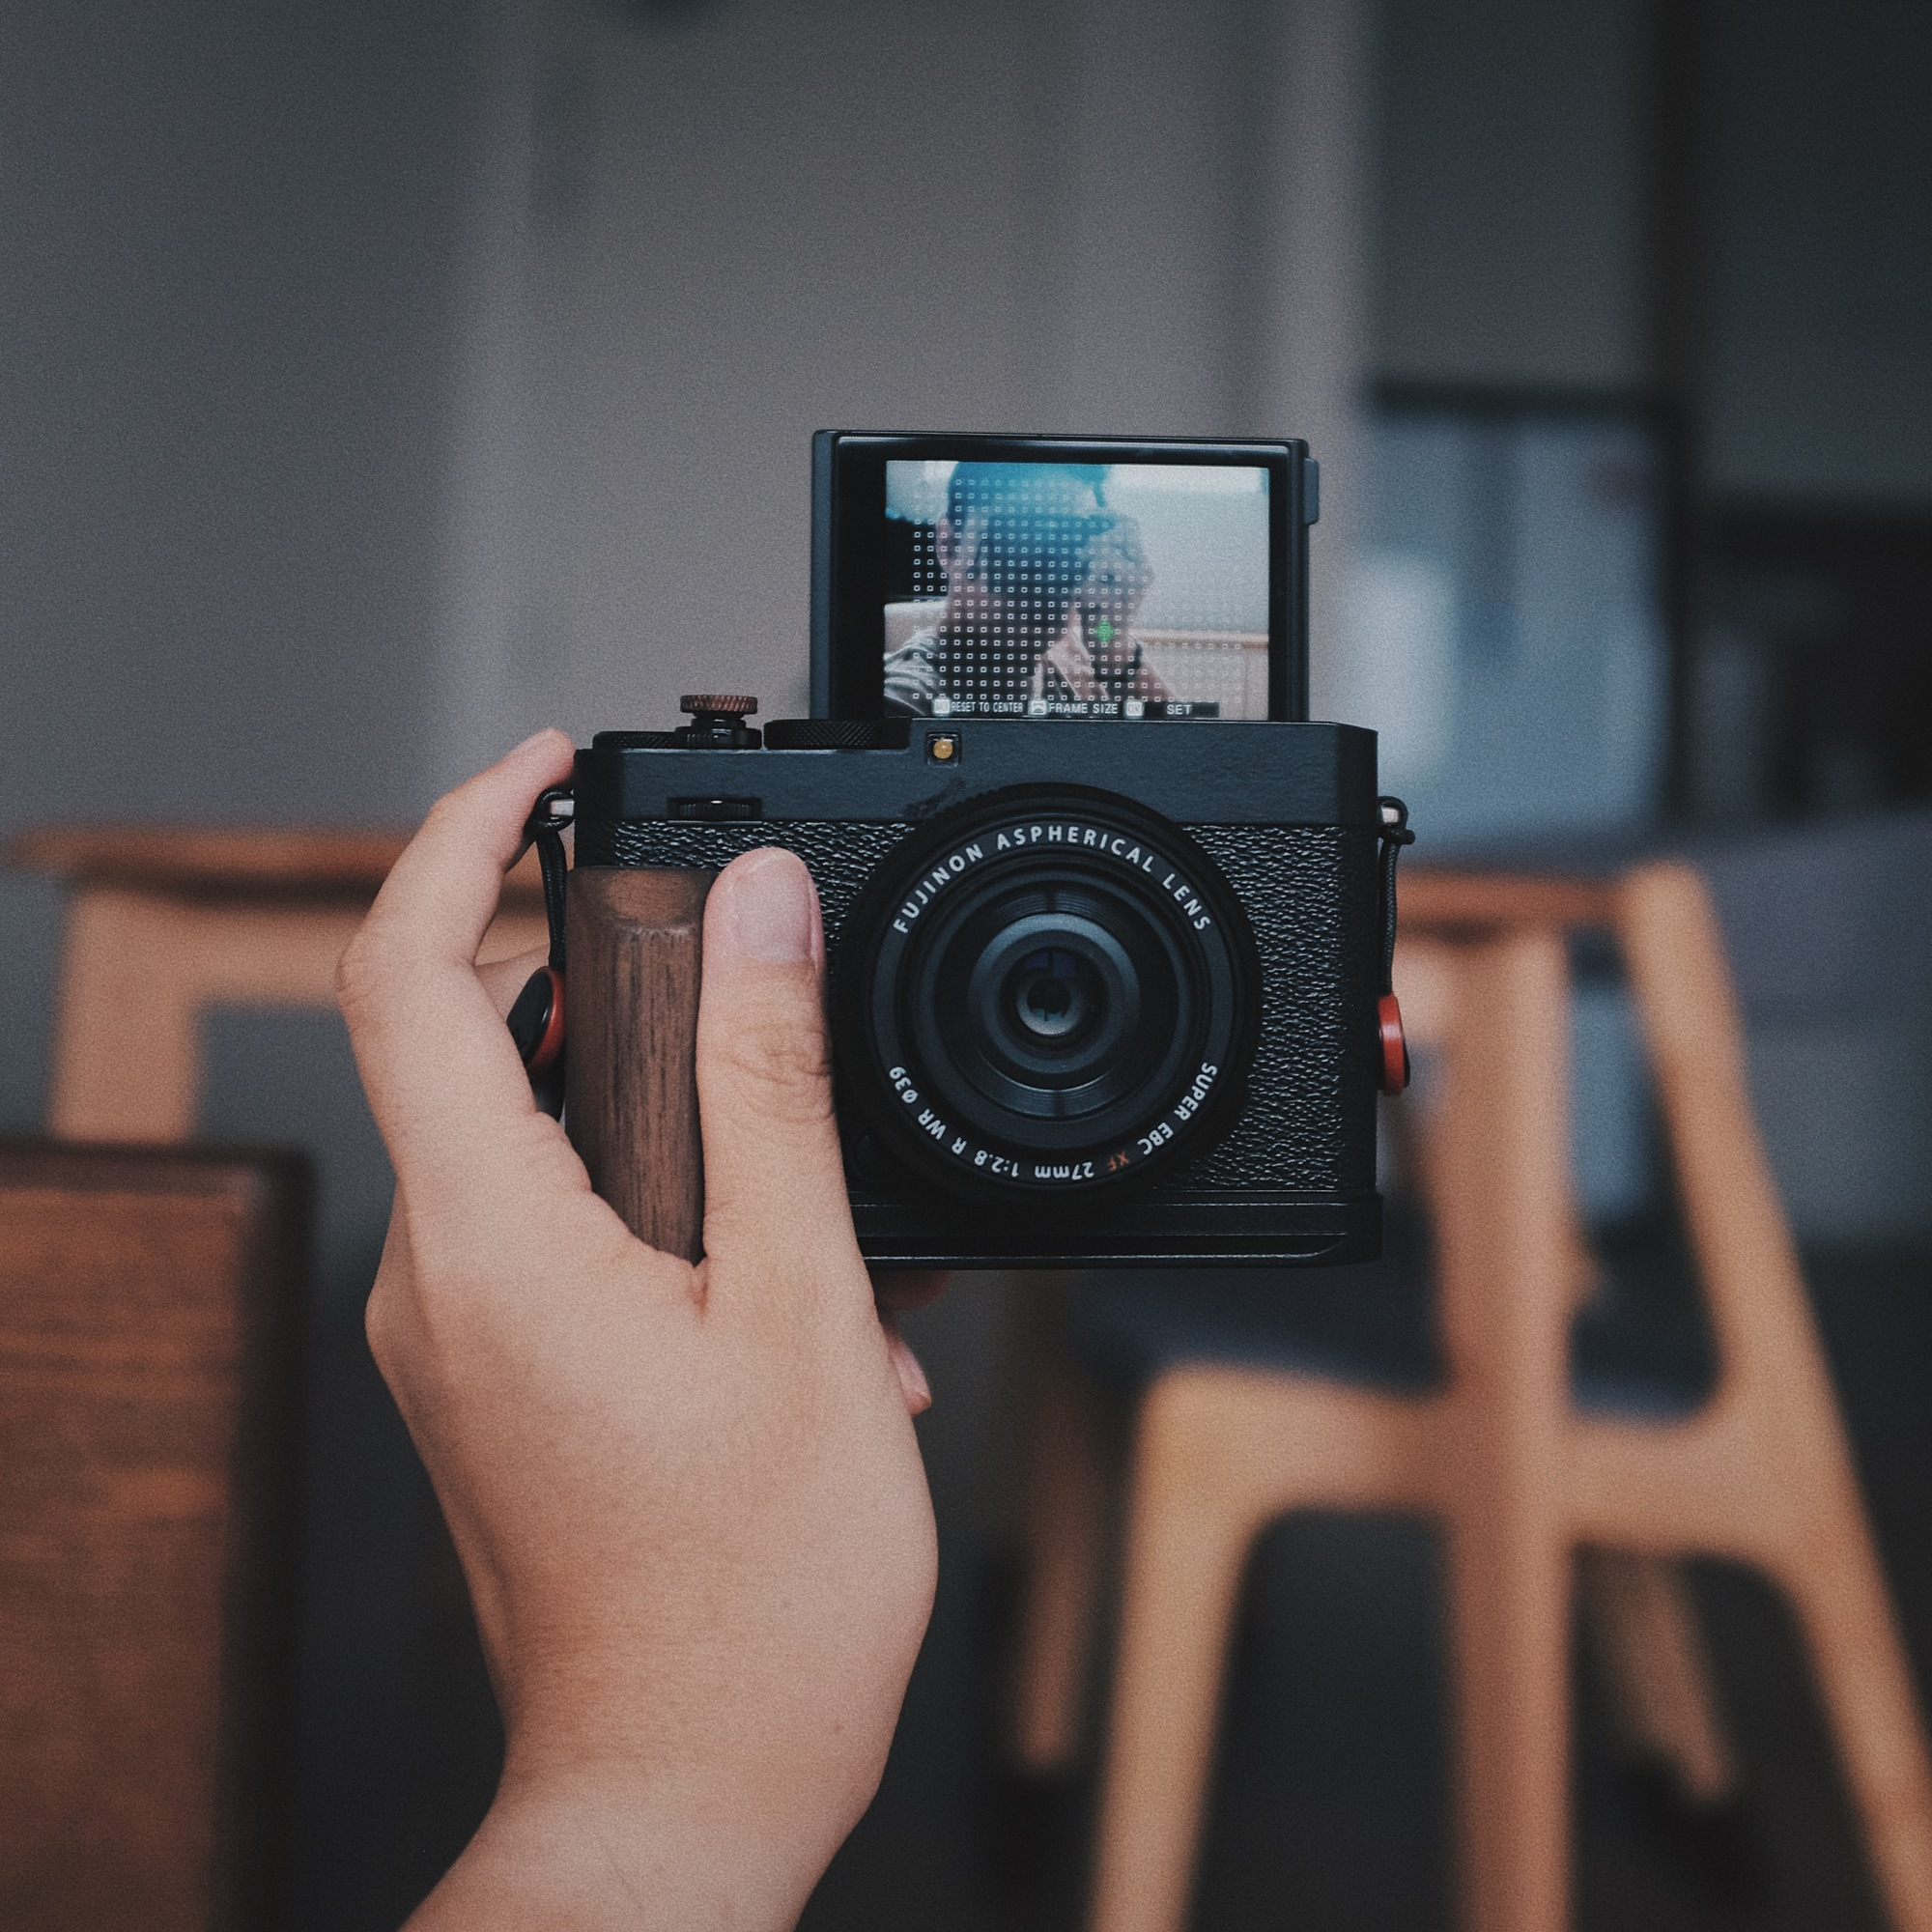
\includegraphics[width=\linewidth]{\envfinaldir/coverpic-prod.jpg}\par
            % \vskip 30pt
            \vfill

            \normalsize\rmfamily\scshape
            \copyright{} The Web Digest Project \hfill\large \envdatestr
        \end{center}
    \end{titlepage}
    % \restoregeometry
}
\newcommand{\simplehref}[1]{%
    \textcolor{blue!80!green}{\href{#1}{#1}}%
}
\renewcommand{\contentsname}{\center\Huge\sffamily\bfseries Contents\par\vskip 20pt}
\newcounter{ipartcounter}
\setcounter{ipartcounter}{0}
\newcommand{\ipart}[1]{
    % \vskip 20pt
    \clearpage
    \stepcounter{ipartcounter}
    \phantomsection
    \addcontentsline{toc}{chapter}{#1}
    % \begin{center}
    %     \Huge
    %     \sffamily\bfseries
    %     #1
    % \end{center}
    % \vskip 20pt plus 7pt
}
\newcounter{ichaptercounter}
\setcounter{ichaptercounter}{0}
\newcommand{\ichapter}[1]{
    % \vskip 20pt
    \clearpage
    \stepcounter{ichaptercounter}
    \phantomsection
    \addcontentsline{toc}{section}{\numberline{\arabic{ichaptercounter}}#1}
    \begin{center}
        \Huge
        \sffamily\bfseries
        #1
    \end{center}
    \vskip 20pt plus 7pt
}
\newcommand{\entrytitlefont}[1]{\subsection*{\raggedright\Large\sffamily\bfseries#1}}
\newcommand{\entryitemGeneric}[2]{
    % argv: title, url
    \parbox{\linewidth}{
        \entrytitlefont{#1}\par\vskip 5pt
        \footnotesize\ttfamily\mdseries
        \simplehref{#2}
    }\vskip 11pt plus 11pt minus 1pt
}
\newcommand{\entryitemGithub}[3]{
    % argv: title, url, desc
    \parbox{\linewidth}{
        \entrytitlefont{#1}\par\vskip 5pt
        \footnotesize\ttfamily\mdseries
        \simplehref{#2}\par\vskip 5pt
        \small\rmfamily\mdseries#3
    }\vskip 11pt plus 11pt minus 1pt
}
\newcommand{\entryitemAp}[3]{
    % argv: title, url, desc
    \parbox{\linewidth}{
        \entrytitlefont{#1}\par\vskip 5pt
        \footnotesize\ttfamily\mdseries
        \simplehref{#2}\par\vskip 5pt
        \small\rmfamily\mdseries#3
    }\vskip 11pt plus 11pt minus 1pt
}
\newcommand{\entryitemHackernews}[3]{
    % argv: title, hnurl, rawurl
    % \parbox{\linewidth}{
    %     \entrytitlefont{#1}\par\vskip 5pt
    %     \footnotesize\ttfamily\mdseries
    %     \simplehref{#3}\par
    %     \textcolor{black!50}{\href{#2}{#2}}
    % }\vskip 11pt plus 11pt minus 1pt
    \begin{minipage}{\linewidth}
            \entrytitlefont{#1}\par\vskip 5pt
            \footnotesize\ttfamily\mdseries
            \simplehref{#3}\par
            \textcolor{black!50}{\href{#2}{#2}}
    \end{minipage}\par\vskip 11pt plus 11pt minus 1pt
}







\begin{document}

\makeheader

\tableofcontents\clearpage




\ipart{Developers}
\ichapter{Hacker News}
\entryitemTwoLinks{iOS Kindle app now has a `get book' button after changes to App Store rules}{https://news.ycombinator.com/item?id=43909432}{https://www.theverge.com/news/661719/amazon-app-ios-apple-iphone-ipad-kindle-buy-books}

\entryitemTwoLinks{TeleMessage, used by Trump officials, can access plaintext chat logs}{https://news.ycombinator.com/item?id=43909220}{https://micahflee.com/despite-misleading-marketing-israeli-company-telemessage-used-by-trump-officials-can-access-plaintext-chat-logs/}

\entryitemTwoLinks{Matt Godbolt sold me on Rust by showing me C++}{https://news.ycombinator.com/item?id=43907820}{https://www.collabora.com/news-and-blog/blog/2025/05/06/matt-godbolt-sold-me-on-rust-by-showing-me-c-plus-plus/}

\entryitemTwoLinks{Curl: We still have not seen a valid security report done with AI help}{https://news.ycombinator.com/item?id=43907376}{https://www.linkedin.com/posts/danielstenberg\_hackerone-curl-activity-7324820893862363136-glb1}

\entryitemTwoLinks{Launch HN: Exa (YC S21) – The web as a database}{https://news.ycombinator.com/item?id=43906841}{https://news.ycombinator.com/item?id=43906841}

\entryitemTwoLinks{Show HN: Sheet Music in Smart Glasses}{https://news.ycombinator.com/item?id=43906442}{https://news.ycombinator.com/item?id=43906442}

\entryitemTwoLinks{Gemini 2.5 Pro Preview}{https://news.ycombinator.com/item?id=43906018}{https://developers.googleblog.com/en/gemini-2-5-pro-io-improved-coding-performance/}

\entryitemTwoLinks{Show HN: Clippy – 90s UI for local LLMs}{https://news.ycombinator.com/item?id=43905942}{https://felixrieseberg.github.io/clippy/}

\entryitemTwoLinks{Accents in latent spaces: How AI hears accent strength in English}{https://news.ycombinator.com/item?id=43905299}{https://accent-strength.boldvoice.com/}

\entryitemTwoLinks{Nnd – a TUI debugger alternative to GDB, LLDB}{https://news.ycombinator.com/item?id=43905185}{https://github.com/al13n321/nnd}

\entryitemTwoLinks{OpenAI reaches agreement to buy Windsurf for around \$3B}{https://news.ycombinator.com/item?id=43904233}{https://www.bloomberg.com/news/articles/2025-05-06/openai-reaches-agreement-to-buy-startup-windsurf-for-3-billion}

\entryitemTwoLinks{New studies offer insight into Lyme disease's treatment, lingering symptoms}{https://news.ycombinator.com/item?id=43903959}{https://news.northwestern.edu/stories/2025/04/taking-the-bite-out-of-lyme-disease/}

\entryitemTwoLinks{Memory-safe sudo to become the default in Ubuntu}{https://news.ycombinator.com/item?id=43903853}{https://trifectatech.org/blog/memory-safe-sudo-to-become-the-default-in-ubuntu/}

\entryitemTwoLinks{Getting things ``done'' in large tech companies}{https://news.ycombinator.com/item?id=43903741}{https://www.seangoedecke.com/getting-things-done/}

\entryitemTwoLinks{Design and evaluation of a parrot-to-parrot video-calling system (2023)}{https://news.ycombinator.com/item?id=43903728}{https://www.smithsonianmag.com/smart-news/scientists-taught-pet-parrots-to-video-call-each-other-and-the-birds-loved-it-180982041/}

\entryitemTwoLinks{The Turkish İ Problem and Why You Should Care (2012)}{https://news.ycombinator.com/item?id=43902869}{https://haacked.com/archive/2012/07/05/turkish-i-problem-and-why-you-should-care.aspx/}

\entryitemTwoLinks{Sneakers (1992) – 4K makeover sourced from the original camera negative}{https://news.ycombinator.com/item?id=43902263}{https://www.blu-ray.com/movies/Sneakers-4K-Blu-ray/343185/}

\entryitemTwoLinks{The curse of knowing how, or; fixing everything}{https://news.ycombinator.com/item?id=43902212}{https://notashelf.dev/posts/curse-of-knowing}

\entryitemTwoLinks{An appeal to Apple from Anukari}{https://news.ycombinator.com/item?id=43901619}{https://anukari.com/blog/devlog/an-appeal-to-apple}

\entryitemTwoLinks{Critical CSS}{https://news.ycombinator.com/item?id=43901495}{https://critical-css-extractor.kigo.studio/}\ichapter{Phoronix}
\entryitemGeneric{\hskip 0pt{}Valve Releases Updated Proton 10.0 Beta For Testing}{https://www.phoronix.com/news/Proton-10.0-Beta-Updated}

\entryitemGeneric{\hskip 0pt{}RISC-V LLVM Scheduler Tuning For SpacemiT-X60 On Clang Yields 4~18\% Speedups}{https://www.phoronix.com/news/SpacemiT-X60-LLVM-Scheduler}

\entryitemGeneric{\hskip 0pt{}Microsoft Welcomes Fedora Linux As An Official WSL Distro}{https://www.phoronix.com/news/Fedora-Linux-Official-WSL}

\entryitemGeneric{\hskip 0pt{}Intel's Clear Linux Demonstrates Software Optimization Benefits On AMD EPYC 9005 Series}{https://www.phoronix.com/review/amd-epyc-mid2025-linux}

\entryitemGeneric{\hskip 0pt{}Ampere Computing Soft Announces AmpereOne M With 12 Channel DDR5 Memory}{https://www.phoronix.com/news/AmpereOne-M-Soft-Announcement}

\entryitemGeneric{\hskip 0pt{}Kurchu Tool Taking Shape For Assembling Fedora / CentOS Linux Distro ISOs}{https://www.phoronix.com/news/CentOS-Kurchu}

\entryitemGeneric{\hskip 0pt{}Ubuntu 25.10 Plans To Use sudo-rs By Default For Memory-Safe, Rust-Based sudo}{https://www.phoronix.com/news/Ubuntu-25.10-sudo-rs-Default}

\entryitemGeneric{\hskip 0pt{}PoCL 7.0 RC1 Released With Official OpenCL 3.0 Conformance On CPUs \& Level Zero}{https://www.phoronix.com/news/PoCL-7.0-RC1-Released}

\entryitemGeneric{\hskip 0pt{}Btrfs "CLEAR\_FREE" Looks Like It Will Be Ready For Linux 6.16}{https://www.phoronix.com/news/Btrfs-CLEAR\_FREE-In-Next}\ichapter{Dribbble}
\entryitemGeneric{\hskip 0pt{}AI Security}{https://dribbble.com/shots/25987123-AI-Security}

\entryitemGeneric{\hskip 0pt{}Fiyah > Hot Sauces Line}{https://dribbble.com/shots/25989187-Fiyah-Hot-Sauces-Line}

\entryitemGeneric{\hskip 0pt{}Crypto Portfolio Tracker App}{https://dribbble.com/shots/25988631-Crypto-Portfolio-Tracker-App}

\entryitemGeneric{\hskip 0pt{}Just a Hippo}{https://dribbble.com/shots/25988582-Just-a-Hippo}

\entryitemGeneric{\hskip 0pt{}Quartz Wordmark Logo}{https://dribbble.com/shots/25985137-Quartz-Wordmark-Logo}

\entryitemGeneric{\hskip 0pt{}Fianance Landing Page}{https://dribbble.com/shots/25980595-Fianance-Landing-Page}

\entryitemGeneric{\hskip 0pt{}Heliara}{https://dribbble.com/shots/25983106-Heliara}

\entryitemGeneric{\hskip 0pt{}UI/UX Design for AURA — your personal AI assistant}{https://dribbble.com/shots/25982086-UI-UX-Design-for-AURA-your-personal-AI-assistant}

\entryitemGeneric{\hskip 0pt{}Envisioning the future}{https://dribbble.com/shots/25985271-Envisioning-the-future}

\entryitemGeneric{\hskip 0pt{}GOCCO Wordmark}{https://dribbble.com/shots/25984476-GOCCO-Wordmark}

\entryitemGeneric{\hskip 0pt{}Lume}{https://dribbble.com/shots/25978139-Lume}

\entryitemGeneric{\hskip 0pt{}Illustration}{https://dribbble.com/shots/25975830-Illustration}

\entryitemGeneric{\hskip 0pt{}Medical Landing Page Design}{https://dribbble.com/shots/25971117-Medical-Landing-Page-Design}

\entryitemGeneric{\hskip 0pt{}Onboarding illustrations set on UI8}{https://dribbble.com/shots/25973282-Onboarding-illustrations-set-on-UI8}

\entryitemGeneric{\hskip 0pt{}Mozambique}{https://dribbble.com/shots/25970792-Mozambique}

\entryitemGeneric{\hskip 0pt{}Order details modal calendar dashboard}{https://dribbble.com/shots/25966379-Order-details-modal-calendar-dashboard}

\entryitemGeneric{\hskip 0pt{}W Letter Logo Concept}{https://dribbble.com/shots/25970255-W-Letter-Logo-Concept}

\entryitemGeneric{\hskip 0pt{}Phantom apple watch}{https://dribbble.com/shots/25967884-Phantom-apple-watch}

\entryitemGeneric{\hskip 0pt{}South Africa}{https://dribbble.com/shots/25967008-South-Africa}

\entryitemGeneric{\hskip 0pt{}Startup UI UX Design, User Interface Experience for Tempest}{https://dribbble.com/shots/25960670-Startup-UI-UX-Design-User-Interface-Experience-for-Tempest}

\entryitemGeneric{\hskip 0pt{}Tornado}{https://dribbble.com/shots/25964784-Tornado}

\entryitemGeneric{\hskip 0pt{}P - Style exploration}{https://dribbble.com/shots/25965406-P-Style-exploration}

\entryitemGeneric{\hskip 0pt{}Branding for NeoAI – your intelligent personal assistant}{https://dribbble.com/shots/25963980-Branding-for-NeoAI-your-intelligent-personal-assistant}

\entryitemGeneric{\hskip 0pt{}Tech illustration pack on UI8}{https://dribbble.com/shots/25948747-Tech-illustration-pack-on-UI8}


\ipart{Developers~~~~(zh-Hans)}
\ichapter{Solidot}
\entryitemGeneric{\hskip 0pt{}Half-Life 3 可能年内宣布}{https://www.solidot.org/story?sid=81214}

\entryitemGeneric{\hskip 0pt{}洗衣机难以真正消毒}{https://www.solidot.org/story?sid=81213}

\entryitemGeneric{\hskip 0pt{}日本 15 岁以下儿童首次跌破 1400 万}{https://www.solidot.org/story?sid=81212}

\entryitemGeneric{\hskip 0pt{}特朗普政府大幅削减 NASA 预算,将重心转移到火星}{https://www.solidot.org/story?sid=81211}

\entryitemGeneric{\hskip 0pt{}北美鸟类加快消减 }{https://www.solidot.org/story?sid=81210}

\entryitemGeneric{\hskip 0pt{}Threads 用户数突破 3.5 亿}{https://www.solidot.org/story?sid=81209}

\entryitemGeneric{\hskip 0pt{}Mozilla 高管称没有 Google 的默认搜索交易它会倒闭}{https://www.solidot.org/story?sid=81208}\ichapter{V2EX}
\entryitemGeneric{\hskip 0pt{}[问与答] 玩 hifi 或者音响的 v 友求指导}{https://www.v2ex.com/t/1130038}

\entryitemGeneric{\hskip 0pt{}[分享发现] 没想到 Cursor 也有教育优惠了}{https://www.v2ex.com/t/1130037}

\entryitemGeneric{\hskip 0pt{}[VPS] 有哪些关机不计费的云厂商?}{https://www.v2ex.com/t/1130036}

\entryitemGeneric{\hskip 0pt{}[OpenAI] gemini 2.5pro 核心开发人员是不是有毛子?一遇到疑难杂症进展到比较迷茫的阶段就全面英文切俄文}{https://www.v2ex.com/t/1130035}

\entryitemGeneric{\hskip 0pt{}[Apple] 发现一个 safari 长按图片小技巧}{https://www.v2ex.com/t/1130033}

\entryitemGeneric{\hskip 0pt{}[分享创造] 感谢「[开源分享/视频演示] 我开发的一款 Chrome/Edge 插件:公众号阅读增强器」}{https://www.v2ex.com/t/1130032}

\entryitemGeneric{\hskip 0pt{}[Apple] 「震撼发布」 分享一些个人收集的高性能全 USB-C 口充电头(欢迎补充)}{https://www.v2ex.com/t/1130031}

\entryitemGeneric{\hskip 0pt{}[问与答] 各位佬,闲置游戏本如何不吃灰废物利用}{https://www.v2ex.com/t/1130030}

\entryitemGeneric{\hskip 0pt{}[问与答] 大家用竖屏显示器吗? 27 寸我试了试,太大了。求推荐 24 寸 4k 显示器~~~}{https://www.v2ex.com/t/1130029}

\entryitemGeneric{\hskip 0pt{}[信息安全] 你听我说,这个仿闲鱼诈骗平台是这样的。}{https://www.v2ex.com/t/1130028}

\entryitemGeneric{\hskip 0pt{}[分享创造] 静态网页"小废物``又添一枚,就是找彩蛋的``小游戏''!}{https://www.v2ex.com/t/1130027}

\entryitemGeneric{\hskip 0pt{}[酷工作] [北京] 元火花-大模型应用初创公司招聘 - 软件工程师(前端、后端、算法、数据、Infra 等)}{https://www.v2ex.com/t/1130025}

\entryitemGeneric{\hskip 0pt{}[分享创造] 我过 iframe 的方式嵌入了一个在线地理猜测游戏,叫 GeoGuessr,你可以通过视频里街景周围环境来推测你的位置。}{https://www.v2ex.com/t/1130024}

\entryitemGeneric{\hskip 0pt{}[酷工作] [杭州] [1-5 年/14-25k] AI 产品经理 [8 小时不加班/AI SaaS]}{https://www.v2ex.com/t/1130023}

\entryitemGeneric{\hskip 0pt{}[分享发现] 申请收录个人博客: 敲代码的卡卡罗特}{https://www.v2ex.com/t/1130022}

\entryitemGeneric{\hskip 0pt{}[程序员] 如何将 html 页面地图保存成大分辨率图片?}{https://www.v2ex.com/t/1130021}

\entryitemGeneric{\hskip 0pt{}[分享创造] MacOS 上用头来控制鼠标滚动 ----- 开源一款可能缓解程序员颈椎病的软件}{https://www.v2ex.com/t/1130020}

\entryitemGeneric{\hskip 0pt{}[Windows] Windows 11 记事本要支持 Markdown 了}{https://www.v2ex.com/t/1130019}

\entryitemGeneric{\hskip 0pt{}[Grand Theft Auto] GTA6 预告片 2}{https://www.v2ex.com/t/1130018}

\entryitemGeneric{\hskip 0pt{}[酷工作] [杭州] [2-8 年/18-28k] Golang 高级后端工程师 [8 小时不加班/AI SaaS]}{https://www.v2ex.com/t/1130017}

\entryitemGeneric{\hskip 0pt{}[程序员] 大家平时都用什么 json 插件}{https://www.v2ex.com/t/1130016}

\entryitemGeneric{\hskip 0pt{}[问与答] 求职分析🧐}{https://www.v2ex.com/t/1130015}

\entryitemGeneric{\hskip 0pt{}[宽带症候群] HKBN 的企业宽带光猫有可能替换成猫棒,甚至普通的光模块吗?}{https://www.v2ex.com/t/1130014}

\entryitemGeneric{\hskip 0pt{}[音乐] 关于正版音乐(Hi-res)购买的疑问}{https://www.v2ex.com/t/1130013}

\entryitemGeneric{\hskip 0pt{}[程序员] Windsurf 反代配置,支持 tab 自动补全}{https://www.v2ex.com/t/1130009}

\entryitemGeneric{\hskip 0pt{}[问与答] Apple 美区活动:白嫖三个月 Apple tv+和 Apple music}{https://www.v2ex.com/t/1130008}

\entryitemGeneric{\hskip 0pt{}[生活] 有时候遇到小问题,还是自己下手解决来的比较快}{https://www.v2ex.com/t/1130007}

\entryitemGeneric{\hskip 0pt{}[程序员] mac 使用 brew 安装 mysql,登录时报错: ERROR 1045: Access denied for user `root`@`localhost` (using password: YES)}{https://www.v2ex.com/t/1130005}

\entryitemGeneric{\hskip 0pt{}[云计算] 腾讯云 CVM SA9 出了}{https://www.v2ex.com/t/1130004}

\entryitemGeneric{\hskip 0pt{}[云计算] 腾讯云的轻量居然都有 AMD EPYC 7K83 的机型了}{https://www.v2ex.com/t/1130002}

\entryitemGeneric{\hskip 0pt{}[问与答] 求助群友,怎么让 MBA M3 带两个 4k 显示器,其中一个是高刷}{https://www.v2ex.com/t/1130000}

\entryitemGeneric{\hskip 0pt{}[宽带症候群] 移动宽带最近真是难用}{https://www.v2ex.com/t/1129999}

\entryitemGeneric{\hskip 0pt{}[问与答] 长期使用的外币虚拟卡求推荐}{https://www.v2ex.com/t/1129997}

\entryitemGeneric{\hskip 0pt{}[macOS] 用触摸板怎么选择大面积的文本?}{https://www.v2ex.com/t/1129995}

\entryitemGeneric{\hskip 0pt{}[职场话题] 底层前端未来的出路在哪里呢?}{https://www.v2ex.com/t/1129994}

\entryitemGeneric{\hskip 0pt{}[职场话题] 哺乳期拖欠工资怎么解决}{https://www.v2ex.com/t/1129993}

\entryitemGeneric{\hskip 0pt{}[程序员] 让智能更生动·让创想更自由,硬件资料可以直接生产,软件代码可以直接编译,服务器可以自已搭建,开源玩转情感交互新世代}{https://www.v2ex.com/t/1129992}

\entryitemGeneric{\hskip 0pt{}[macOS] brew uninstall --zap <cask> 报权限的错, 有人和我一样吗?}{https://www.v2ex.com/t/1129991}

\entryitemGeneric{\hskip 0pt{}[旅行] 泰国曼谷红灯区真不咋地}{https://www.v2ex.com/t/1129990}

\entryitemGeneric{\hskip 0pt{}[投资] 分享两个美股 etf}{https://www.v2ex.com/t/1129987}

\entryitemGeneric{\hskip 0pt{}[职场话题] 准备回重庆了, 转什么技术好点}{https://www.v2ex.com/t/1129986}

\entryitemGeneric{\hskip 0pt{}[宽带症候群] 有点想办抖音刷到的 360/年联通宽带 求骂醒}{https://www.v2ex.com/t/1129985}

\entryitemGeneric{\hskip 0pt{}[问与答] 帝都注册的公司,注册地址是挂靠的地址, 官网被挂隐藏链接, 网安通知整改怎么处理?}{https://www.v2ex.com/t/1129981}

\entryitemGeneric{\hskip 0pt{}[问与答] PDD mac air m4 丐版 5798 能上车吗?}{https://www.v2ex.com/t/1129980}

\entryitemGeneric{\hskip 0pt{}[V2EX] safari 的奇怪触发逻辑}{https://www.v2ex.com/t/1129979}

\entryitemGeneric{\hskip 0pt{}[问与答] 澳门各大娱乐公司的开发团队水平如何?}{https://www.v2ex.com/t/1129976}

\entryitemGeneric{\hskip 0pt{}[酷工作] 招聘帖: flutter、pm、golang、web、运维等,广州、上海}{https://www.v2ex.com/t/1129975}

\entryitemGeneric{\hskip 0pt{}[macOS] Mac 微信双开的问题}{https://www.v2ex.com/t/1129974}

\entryitemGeneric{\hskip 0pt{}[Apple] Mac mini or i5 14600kf+5070}{https://www.v2ex.com/t/1129972}

\entryitemGeneric{\hskip 0pt{}[Windows] win11 声卡安装不上}{https://www.v2ex.com/t/1129970}


\ipart{Generic News}
\ichapter{联合早报}
\entryitemWithDescription{黎康:魔都的B面}{https://www.zaobao.com/news/china/story20250426-6241474}{``确实这几年上海的城市公共建设很好,但你有没有去看过一些老旧小区的环境?小区里电线横飞,绿化基本毫无规划;进入楼道,你会感觉回到20年前\ldots\ldots'' 上一篇``早点------沪上闲语''发表后,收到一封读者来信。这位上海市民告诉我,在装点城市门面的郁金香背后,如果走进上海的老旧小区,会看到这座城市的另一面……}

\entryitemWithDescription{新闻人间:从``不懂球的胖子''到改革推手——刘国梁}{https://www.zaobao.com/news/china/story20250426-6238850}{中国乒乓球协会星期三(4月23日)突然宣布,刘国梁主动辞去主席一职。这一消息迅速引发体坛热议,有球迷为他的离开感到惋惜,也有体育评论员开始审视他在任期内的功与过。 刘国梁自2018年起担任乒协主席,如今在第二任期尚未结束之际中途请辞,外界难免有诸多猜测。星期三当天,他以主席身份在乒协会议上作最后一次发言时,几度哽咽,甚至当场落泪。 他在记者会上透露,早在去年巴黎奥运会结束后,便已向上级表达了去意……}

\entryitemWithDescription{中国据报考虑暂停加征部分美国产品125\%关税}{https://www.zaobao.com/news/china/story20250425-6245926}{中国政府据报考虑暂停对部分美国进口产品加征125\%的关税,受访学者认为此举主要考虑中国企业的生存需要,与中美是否开启贸易谈判无关。 据彭博社引述知情人士报道,中国政府正考虑取消对美国的医疗设备,以及乙烷等工业化学品加征的报复性关税。中国是全球最大的塑料制造国,但部分工厂依赖从美国进口的乙烷。中国医院也需要美国生产的磁共振成像和超声仪器等医疗设备。 知情人士称,飞机租赁也可能豁免关税……}

\entryitemWithDescription{中国美国商会白皮书:五分之一美企不再视中国为优先投资地}{https://www.zaobao.com/news/china/story20250425-6245113}{中国美国商会的调查显示,五分之一的在华美国企业不再将中国列为优先的投资目的地。 该商会星期五(4月25日)发布由100余名中国美国商会会员企业代表共同撰写的2025年《美国企业在中国白皮书》。 白皮书指出,中美两国关系日益紧张,已连续五年成为在华美资企业面临的首要商业挑战,超过了合规风险和来自中国企业的竞争压力……}

\entryitemWithDescription{中国发布生态调查报告 称菲律宾捕捞现场发现人为弃置物}{https://www.zaobao.com/news/china/story20250425-6244616}{(北京讯)中国多家自然生态机构星期五(4月25日)联合公布一份调查报告,评估铁线礁、牛轭礁珊瑚礁的生态系统状况,称菲律宾所谓``中国在铁线礁倾倒珊瑚碎屑等言论''毫无科学和事实依据。 中国自然资源部微信公号分别发表了这份题为《铁线礁、牛轭礁珊瑚礁生态系统调查报告》的中英文版本,参与编制的机构包括中国自然资源部南海发展研究院、南海生态中心等……}

\entryitemWithDescription{香港公共场所明年起设更多禁烟区 违例罚款提高一倍}{https://www.zaobao.com/news/china/story20250425-6245064}{为了进一步降低吸烟率,香港特区政府将由明年起在更多公共场所设立禁烟区,并把违例吸烟的罚款金额提高一倍至3000港元(508新元)。 相关条例草案星期五(4月25日)刊宪,列明从明年元旦起,禁止在等候公共交通工具、等候进入电影院、医院、公众游乐场地、体育场等地方的划定范围吸烟。违者罚款由1500港元倍增至3000港元……}

\entryitemWithDescription{两韩国顶尖半导体专家 退休后被中国高校任用}{https://www.zaobao.com/news/china/story20250425-6244895}{(首尔讯)中国正通过从海外引进顶尖人才,与美国争夺高科技主导权。韩国两名``国宝级''顶尖专家退休后在本国受到冷落,未能找到合适研究职位,目前已被中国高等学府任用。 据韩国《中央日报》报道,韩国知名碳纳米管专家李永熙去年11月正式受聘于湖北工业大学半导体与量子研究所……}

\entryitemWithDescription{美国传降对陆关税又强化对台论述 分析:谈判或拿台湾当筹码}{https://www.zaobao.com/news/china/story20250425-6244227}{华盛顿释出降低对华关税信号、寻求谈判之际,美国星期三(4月23日)首次在联合国安理会批评北京误用联大2758号决议;更在同一天派遣军舰穿越台湾海峡。受访学者分析,这些作为现阶段暂与关税战没有直接关联,但不排除美国总统特朗普接下来可能利用台湾问题作为对华谈判筹码。 特朗普本周透露考虑大幅度降低对华关税,希望与中国达成``公平的协议'',同时又声称美国每天都同中国直接联系……}

\entryitemWithDescription{韩咏红:特朗普关税从``解放日''走到``妥协日''了?}{https://www.zaobao.com/news/china/story20250425-6240846}{美国总统特朗普在4月2日宣布对等关税政策,短短20天后,特朗普的高姿态已难以为继。特朗普在4月9日就已调整过一次战术,暂缓对其他国家课征对等关税,集中火力单挑中国;而今,特朗普恐怕又要眨眼了,对中国商品课征的145\%关税也可能显著下调。 特朗普近日罕见地对中国伸出橄榄枝,表示考虑大幅度降低对华关税,显露出急于与中国达成协议。但中国偏是表现得不着急……}

\entryitemWithDescription{学者:中国以2+2机制拉拢东南亚国家抗衡美国}{https://www.zaobao.com/news/china/story20250424-6240690}{受访学者分析,在中美关系因贸易战而全面恶化的大背景下,中国正以``外交、国防2+2对话机制''为新抓手,积极拉拢亚细安成员国,以抗衡美国在本区域的影响力,预计中国接下来将推动与更多区域国家建立2+2机制。 中国和印度尼西亚星期一(4月21日)在北京举行外长、防长对话机制下的首次部长级会议,两国在2023年就建立2+2对话机制。中国官方称,这是中国在全球建立的首个部长级2+2机制……}

\entryitemWithDescription{中埃空军首次联训 学者:中国初步具备向中东快速战略投送能力}{https://www.zaobao.com/news/china/story20250424-6240357}{中国空军上周派出多架战斗机、预警机、运输机与空中加油机前往埃及,进行两军首次联训。这是中国空军首次以完整作战体系进行跨洲机动。 受访学者认为,这是中国空军现代化进程的里程碑,有助于发展长途奔袭的技战术;这也标志着中国初步具备向中东进行快速战略投送的能力。 据中国国防部消息,中国与埃及两国空军于4月中旬至5月上旬,在埃及空军基地组织代号为``文明之鹰-2025''的联合训练……}

\entryitemWithDescription{台湾收紧民众申领大陆证照规定 持大陆定居证也将被撤销台湾身份}{https://www.zaobao.com/news/china/story20250424-6239789}{(台北综合讯)台湾再度收紧民众申领中国大陆证照的规定,持有大陆定居证的台湾民众也触犯相关法令,将丧失台湾身份。 综合《旺报》与《联合报》报道,台湾行政院公报显示,陆委会近日对《两岸条例》当中规定发布解释函令称,为确保两岸人员单一身份制度,两岸条例规定台湾人民不得在大陆地区``设有户籍'',或领用大陆地区护照,否则将丧失台湾身份……}

\entryitemWithDescription{神舟二十号成功发射 航天员将开展中国首次涡虫空间再生实验}{https://www.zaobao.com/news/china/story20250424-6239950}{(北京综合讯)中国星期四(4月24日)成功发射神舟二十号载人飞船。三名航天员将在空间站驻留约六个月,并开展中国首次涡虫空间再生实验。 综合新华社、央视新闻和《中国青年报》报道,搭载神舟二十号的长征二号F遥二十运载火箭,星期四下午5时17分在甘肃酒泉卫星发射中心点火发射。约10分钟后,神舟二十号与火箭成功分离,进入预定轨道……}

\entryitemWithDescription{台大罢免升温 朝野对抗加剧}{https://www.zaobao.com/news/china/story20250424-6240062}{台湾两大在野党将携手举办大型造势活动,抗议政府利用司法整肃异己,进行大罢免。兼任民进党主席的总统赖清德则公开肯定公民团体罢免在野党立委的行动影片,检调也持续搜索在野国民党宜兰县党部,朝野对抗情势正逐步升温……}

\entryitemWithDescription{美国国会罕见动用传唤权 调查中国三电信巨头}{https://www.zaobao.com/news/china/story20250424-6239456}{(纽约路透电)美国众议院中国问题特别委员会星期三(4月23日)罕见地动用传唤权,调查中国三大电信公司涉嫌支持中国军方和政府的行为。 据路透社报道,中国移动、中国电信和中国联通三家中国电信巨头收到该委员会的传唤通知,须回答他们是否可通过在美开展的云服务和互联网业务获取美国数据的问题。 美国两党议员持续对被指由中国主导的网络攻击事件表示担忧……}

\entryitemWithDescription{浙江一小学门外发生汽车冲撞人群事件}{https://www.zaobao.com/news/china/story20250424-6238514}{(香港综合讯)中国再发生校园伤人事件,浙江金华一所小学门外星期二(4月22日)放学时有汽车冲撞人群,伤亡人数不明。官方在事发两日后仍未发布通报,中国社媒上的相关信息均被删除。 综合《明报》《南华早报》和网媒``香港01''报道,这起事件发生在金华市苏孟乡中心小学门口,时间是星期二傍晚5时45分左右,正值放学时间。附近商户披露,有多名学生被撞……}

\entryitemWithDescription{学者:关税战伤敌一千自损八百 中美终将找到共处之道}{https://www.zaobao.com/news/china/story20250424-6238821}{美国总统特朗普祭出对等关税将届满一个月,如今传出可能降低对华关税,定居美国的资深华人学者赵全胜指出,中美领导阶层有一批人长期相信对方马上要垮台,但关税战让双方意识到,这无疑是``伤敌一千,自损八百'',因此迟早会找到共处之道。 特朗普4月2日宣布全面实施对等关税,随后在9日紧急暂缓90天,让各国争取与美国谈判的时间与空间,唯独对中国不断加码;北京也不甘示弱,提出相应反制……}

\entryitemWithDescription{打击电诈犯罪扩至纵深地带 缅甸向中国移交920余名嫌犯}{https://www.zaobao.com/news/china/story20250424-6238307}{(北京综合讯)中国与缅甸加大打击电信网络诈骗犯罪合作力度,两国最近一个月的合作执法行动,已从缅北地区扩大到当阳、勐休等缅甸纵深地带。 中国公安部官网星期三(4月23日)通报,缅甸执法部门近日将在当地抓获的920余名中国籍涉诈犯罪嫌疑人,通过云南西双版纳打洛口岸全部移交中国警方。 通报称,缅北电诈犯罪集团遭受重创,但部分涉诈人员为逃避打击,向当阳、勐休等纵深地带转移藏匿,继续实施跨境电诈……}

\entryitemWithDescription{沈泽玮:魔幻山城的中国式现代化演绎}{https://www.zaobao.com/news/china/story20250424-6234868}{时隔12年因工作再访重庆,春夏交替之际迎来烈日当空,与当年冬季旅游行走于山城迷雾的印象截然不同。 5000架无人机灯光秀,既展现科技力量也打造视觉盛宴;科企创始人讲述营商环境不断优化;村委会主任手捧涪陵榨菜分享东方酱腌菜``走出去''成果;火车司机传递通关速度如何带动互联互通跨境贸易;公安局交巡警总队科研处综合科科长讲述数字化赋能超大城市治理;社区党委书记分享中国特色``民主村''的前身今世……}

\entryitemWithDescription{中国网购平台将全面取消``仅退款''}{https://www.zaobao.com/news/china/story20250423-6234242}{在中国官方整治``内卷式竞争''的背景下,中国电商平台将全面取消``仅退款''选项。受访学者认为,此举有助行业回归良性竞争,是对电商市场的一次纠偏。 据《北京商报》报道,拼多多、淘宝、抖音、快手、京东等多个中国电商平台,星期二(4月22日)修改有关``仅退款''的相关条款,消费者申请``退款不退货'',将由商家自主处理……}

\entryitemWithDescription{3月人民币跨境收付占比刷新历史纪录}{https://www.zaobao.com/news/china/story20250423-6233857}{(华盛顿彭博电)随着美元的全球吸引力减弱、中美贸易紧张局势上升,3月中国投资者和贸易公司在国际结算中对人民币的使用大幅增加,创下历史纪录。 彭博社基于中国国家外汇管理局星期二(4月22日)公布的数据计算,3月中国大陆境内个人和机构的跨境业务中,人民币使用占比达 54.3\%,总额7249亿美元(9502亿新元)……}






\clearpage
\leavevmode\vfill
\footnotesize

Copyright \copyright{} 2023-2025 Neruthes and other contributors.

This document is published with CC BY-NC-ND 4.0 license.

The entries listed in this newsletter may be copyrighted by their respective creators.

This newsletter is generated by the Web Digest project.

The newsletters are also delivered via Telegram channel \CJKunderline{\href{https://t.me/webdigestchannel}{https://t.me/webdigestchannel}}.\\
RSS feed is available at \CJKunderline{\href{https://webdigest.pages.dev/rss.xml}{https://webdigest.pages.dev/rss.xml}}.

This newsletter is available in PDF at
\CJKunderline{\href{https://webdigest.pages.dev/}{https://webdigest.pages.dev/}}.

The source code being used to generate this newsletter is available at\\
\CJKunderline{\href{https://github.com/neruthes/webdigest}{https://github.com/neruthes/webdigest}}.

This newsletter is also available in
\CJKunderline{\href{http://webdigest.pages.dev/readhtml/\envyear/WebDigest-20250507.html}{HTML}} and
\CJKunderline{\href{https://github.com/neruthes/webdigest/blob/master/markdown/\envyear/WebDigest-20250507.md}{Markdown}}.


\coverpic{https://unsplash.com/photos/mountains-are-silhouetted-against-a-vibrant-sunrise-6VhIHgqo5qI}{Daniil Silantev}


\end{document}
